\documentclass{article}

\usepackage[utf8]{inputenc}
\usepackage[T1]{fontenc}
\usepackage[english]{babel}

\usepackage{graphicx}
\usepackage{courier}
\usepackage{charter}
\usepackage{xspace}
\usepackage{lipsum}

\usepackage{xcolor}
%\definecolor{butter}{HTML}{FCE94F}
%\definecolor{butter}{HTML}{EDD400}
\definecolor{butter}{HTML}{C4A000}
%\definecolor{orange}{HTML}{FCAF3E}
%\definecolor{orange}{HTML}{F57900}
\definecolor{orange}{HTML}{CE5C00}
%\definecolor{chocolate}{HTML}{E9B96E}
%\definecolor{chocolate}{HTML}{C17D11}
\definecolor{chocolate}{HTML}{8F5902}
%\definecolor{chameleon}{HTML}{8AE234}
%\definecolor{chameleon}{HTML}{73D216}
\definecolor{chameleon}{HTML}{4E9A06}
%\definecolor{skyblue}{HTML}{729FCF}
%\definecolor{skyblue}{HTML}{3465A4}
\definecolor{skyblue}{HTML}{204A87}
%\definecolor{plum}{HTML}{AD7FA8}
%\definecolor{plum}{HTML}{75507B}
\definecolor{plum}{HTML}{5C3566}
%\definecolor{scarletred}{HTML}{EF2929}
%\definecolor{scarletred}{HTML}{CC0000}
\definecolor{scarletred}{HTML}{A40000}
%\definecolor{lightalu}{HTML}{EEEEEC}
%\definecolor{lightalu}{HTML}{D3D7CF}
\definecolor{lightalu}{HTML}{BABDB6}
%\definecolor{darkalu}{HTML}{888A85}
%\definecolor{darkalu}{HTML}{555753}
\definecolor{darkalu}{HTML}{2E3436}

\newcommand{\kwstyle}{}

\usepackage{listings}

\lstset{
%	backgroundcolor=\color{},
	basicstyle=\small\ttfamily\color{black},
%	breakatwhitespace=false,
	breaklines=true,
%	captionpos=b,
	commentstyle=\color{darkalu},
%	deletekeywords={...},
%	escapeinside={\%*}{*)},
%	extendedchars=true,
%	frame=single,
%	keepspaces=true,
	keywordstyle=\kwstyle,
	language=Caml,
%	morekeywords={*,...},
%	numbers=left,
%	numbersep=5pt,
%	numberstyle=\color{},
%	rulecolor=\color{},
%	showspaces=false,
%	showstringspaces=false,
%	showtabs=false,
%	stepnumber=2,
	stringstyle=\color{plum},
	tabsize=2,
%	title=\lstname,
	keywordstyle=[1]\kwstyle\color{chameleon},
	keywordstyle=[2]\kwstyle\color{scarletred},
	keywordstyle=[3]\kwstyle\color{skyblue},
	keywordstyle=[4]\kwstyle\color{butter},
	keywordstyle=[5]\kwstyle\color{skyblue},
	keywordstyle=[6]\kwstyle\color{skyblue},
	keywordstyle=[7]\kwstyle\color{chameleon},
	keywordstyle=[8]\kwstyle\color{butter},
	keywordstyle=[9]\kwstyle\color{butter},
	keywords=[1]{let,val,method,in,and,rec,private,virtual,constraint},
	keywords=[2]{type,open,class,module,exception,external},
	keywords=[3]{fun,function,functor,match,try,with},
	keywords=[4]{as,when,of},
	keywords=[5]{if,then,else},
	keywords=[6]{begin,end,object,struct,sig,for,while,do,done,to,downto},
	keywords=[7]{true,false},
	keywords=[8]{include,inherit,initializer},
	keywords=[9]{new,ref,mutable,lazy,assert,raise},
}

\lstset{literate=
	{0}{{{\kwstyle\color{plum}0}}}1 {0.}{{{\kwstyle\color{plum}0.}}}2
	{1}{{{\kwstyle\color{plum}1}}}1 {1.}{{{\kwstyle\color{plum}1.}}}2
	{2}{{{\kwstyle\color{plum}2}}}1 {2.}{{{\kwstyle\color{plum}2.}}}2
	{3}{{{\kwstyle\color{plum}3}}}1 {3.}{{{\kwstyle\color{plum}3.}}}2
	{4}{{{\kwstyle\color{plum}4}}}1 {4.}{{{\kwstyle\color{plum}4.}}}2
	{5}{{{\kwstyle\color{plum}5}}}1 {5.}{{{\kwstyle\color{plum}5.}}}2
	{6}{{{\kwstyle\color{plum}6}}}1 {6.}{{{\kwstyle\color{plum}6.}}}2
	{7}{{{\kwstyle\color{plum}7}}}1 {7.}{{{\kwstyle\color{plum}7.}}}2
	{8}{{{\kwstyle\color{plum}8}}}1 {8.}{{{\kwstyle\color{plum}8.}}}2
	{9}{{{\kwstyle\color{plum}9}}}1 {9.}{{{\kwstyle\color{plum}9.}}}2
	{->}{{{\kwstyle\color{chameleon}$\rightarrow$}}}2
}


%\usepackage{appendix}
\usepackage[toc, nonumberlist, nopostdot]{glossaries}
\loadglsentries{glossary}
\makeglossaries

%\usepackage{ulem}
\usepackage[colorlinks=true, citecolor=black, linkcolor=black, urlcolor=blue]{hyperref}

\usepackage{enumitem}
\setlist{itemsep=0mm}

\usepackage{hyphenat}
\renewcommand{\-}{\hyp}

\usepackage{colortbl}

\title{Weak models of data consistency}
\author{Benjamin Farinier}
\date{19/05/2014 -- 15/08/2014}

\newcommand{\irmin}{Irmin\xspace}
\newcommand{\git}{Git\xspace}
\newcommand{\lwt}{Lwt\xspace}
\newcommand{\mercurial}{Mercurial\xspace}
\newcommand{\mirage}{Mirage\xspace}
\newcommand{\ocaml}{OCaml\xspace}
\newcommand{\xen}{Xen\xspace}

\newcommand{\code}[1]{\texttt{#1}}

\begin{document}

\maketitle
\tableofcontents

\section[\mirage, an \ocaml-based unikernel system]{\mirage, an \ocaml-based unikernel system\\\normalsize\normalfont(based on the \href{http://openmirage.org}{\texttt{openmirage.org}} website)}

%\subsection{Overview}

\begin{figure}[hbt]
\centering
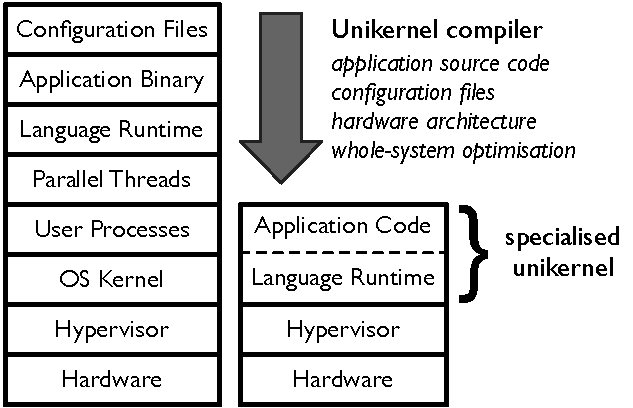
\includegraphics[scale=0.8]{mirage-stack.pdf}
\caption{Contrasting software layers in existing VM appliances vs.
unikernel’s standalone kernel compilation approach.}
\label{miragestackgraph}
\end{figure}

Because they rely on an underlying operating system, most applications that run in the cloud aren't optimised to do so.
Compartmentalisation of large servers into smaller virtual machines has enabled many new businesses to get started and achieve scale.
But many of those virtual machines are single-purpose and yet they contain largely complete operating systems, including their vulnerabilities and bloat.
\mirage represents a new approach where only the necessary components of the OS are included and compiled along with the application into a unikernel.
This results in highly efficient appliances that can be deployed directly to the cloud and embedded devices, with the benefits of reduced costs and increased security and scalability. The figure~\ref{miragestackgraph} explicit the gain of unikernel compared to standard kernels.

\mirage is a \emph{library operating system}\cite{LibraryOperatingSystemsCloud2013} for constructing secure, high-performance network applications across a variety of cloud computing and mobile platforms.
It is based around the \xen hypervisor and the \ocaml langage.
\xen\cite{XenArtVirtualization2003} provides a stable hardware platform, which avoids the need to support the thousands of device drivers found in a traditional OS.
Thanks to \ocaml\cite{CreatingFunctionalInternet2007}, code can be developed in a high-level functional programming language which avoids many of usual flaws.
It is then compiled into a fully-standalone, specialised unikernel which can run directly on \xen hypervisor APIs.
Since \xen powers most public clouds, \mirage lets you deploy your servers more cheaply, securely and faster in any of them.

Due to the small size, it is possible for example to create auto-scaling web-servers with very small footprints.
If a sudden spike in traffic occurs, the web-servers can be configured to create and deploy copies of themselves to service the demand.
This auto-scaling happens so quickly that an incoming connection can trigger the creation of new server and the new server can then handle that request before it times out (which is on the order of milliseconds).
When the demand dies down again, these web-servers can automatically shut themselves down.
This elasticity result in the possibility to precisely meet the demand, avoiding waste of resources.

\paragraph{Towards a distributed database}
As a cloud oriented operating system, \mirage has to deal with distributed system related problems.
One of them is to share data between several devices spread out over a network.
This is the purpose of distributed databases.
\irmin is a portable distributed database written in \ocaml, and designed with  requirements of static type-safety for security and reliability.

%\subsection{Technical background}

%Unikernels are specialised OS kernels written in a high-level language which act as individual software components.
%A full application consists of a set of running unikernels working together as a distributed system.
%These unikerels are based on a radical operating system architecture called library operating system (or libOS).
%
%This architecture is composed of a set of libraries that implement mechanisms, such as those needed to drive hardware or talk network protocols, and a set of policies that enforce access control and isolation in the application layer.
%The libOS architecture has several advantages over more conventional designs.
%For example, when performances are required, a libOS wins by allowing applications to access hardware resources directly without having to make repeated privilege transitions to move data between userspace and kernelspace.
%The libOS architecture has also two big drawbacks.
%First, running multiple applications side by side with strong resource isolation is tricky.
%Second, device drivers must be rewritten to fit the new model.
%
%Happily, OS virtualization overcomes these drawbacks on commodity hardware.
%A libOS running as a VM needs to implement only drivers for these virtual hardware devices and can depend on the hypervisor to achieve the isolation between applications.
%But although OS virtualization avoid the need of rewrite every device drivers, protocol libraries are still needed to replace the services of a traditional operating system.
%
%When most of modern kernels are written in C, \mirage aims to unify these diverse interfaces into a single high-level language, \ocaml. Some of the benefits of such a modern programming languages include:
%
%\begin{itemize}
%	\item \emph{Static type checking}: Compilers catches errors at compile time rather than runtime and reduce vulnerabilities through the lack of memory errors
%	\item \emph{Automatic memory management}: Runtime systems relieve programmers of the burden of allocating and freeing memory, avoiding memory leaks
%	\item \emph{Modules}: Internal implementation details can be abstracted and the scope of a single source-code change can be restricted
%	\item \emph{Metaprogramming}: If the runtime configuration of a system is partially understood at compile time, then a compiler can optimize the program much more than it would normally be able to
%\end{itemize}
%
%Moreover, the \ocaml compiler heavily emphasises static type checking, and the resulting binaries are fast native code with no runtime type information and the module system is among the most powerful in a general-purpose programming language in terms of permitting flexible and safe code reuse and refactoring.
%
%Unikernels are specialised OS kernels written in a high-level language which act as individual software components.
%A full application consists of a set of running unikernels working together as a distributed system.
%These unikerels are based on a radical operating system architecture called library operating system (or libOS)\cite{LibraryOperatingSystemsCloud2013}.
%
%This architecture is composed of a set of libraries that implement mechanisms, such as those needed to drive hardware or talk network protocols.
%When a system component is needed, the developer just has to integrate the corresponding library in its program in order to manipulate the device through the provided interface.
%As a result, only needed components are integrated in the final application.
%
%The libOS architecture has several advantages over more conventional designs.
%For example, when performances are required, a libOS wins by allowing applications to access hardware resources directly without having to make repeated privilege transitions to move data between userspace and kernelspace.
%The libOS architecture has also two big drawbacks.
%First, running multiple applications side by side with strong resource isolation is tricky.
%Second, device drivers must be rewritten to fit the new model.
%Happily, OS virtualization overcomes these drawbacks on commodity hardware.
%Indeed, a libOS running as a VM needs to implement only drivers for these virtual hardware devices and can depend on the hypervisor to achieve the isolation between applications.
%But although OS virtualization avoid the need of rewrite every device drivers, protocol libraries are still needed to replace the services of a traditional operating system.
%
%When most of modern kernels are written in C, \mirage aims to unify these diverse interfaces into a single high-level language, \ocaml.
%Some of the benefits of using \ocaml include:
%
%\begin{itemize}
%	\item It is a full-fledged systems programming language with a flexible model that supports functional, imperative and object-oriented programming
%	\item Some modern features like static type checking, automatic memory management, modules and metaprogramming make unikernels robust\cite{CreatingFunctionalInternet2007} against attacks like memory overflow
%	\item \ocaml has a simple yet high-performance runtime making it an ideal platform for experimenting with the unikernel abstraction that interfaces the runtime with \xen
%	\item Some critical system component of \xen  are implemented in \ocaml, making integration straightforward
%\end{itemize}
%
%\mirage executes \ocaml code over a specialised language runtime modified in two key areas: memory management and concurrency.
%To provide concurrency, \mirage integrates the \lwt cooperative threading library, which provide straight-line control flow for the developer.
%Most scheduling and thread logic is contained in an application library, and can thus be modified by the developer as they see fit\cite{LibraryOperatingSystemsCloud2013}.



\section{\irmin, a large-scale, immutable, branch-consistent storage}

\subsection{Design}

Designing distributed database is an hard problem, mainly because of CAP’s theorem\cite{BrewerConjecture2002} which states that:

\bigskip
\begin{tabular}{|c}
\begin{minipage}{0.9\textwidth}
It is impossible for a distributed system to simultaneously provide all three of the following guarantees:
\begin{enumerate}
	\item \emph{Consistency}: all nodes see the same data at the same time
	\item \emph{Availability}: a guarantee that every request receives a response about whether it was successful or failed
	\item \emph{Partition tolerance}: the system continues to operate despite arbitrary message loss or failure of part of the system.
\end{enumerate} 
\end{minipage}
\end{tabular}
\bigskip

The modern answer to solve this paradox is to maintain availability but relax the consistency model.
Most of the large-scale distributed system assume there is no unique global state of the system, which result in a class of system said to be \emph{eventually consistent}\cite{EventuallyConsistentTransactions2012}.
The approach of \irmin to relax the consistency model is inspired by distributed version control system such as \git and \mercurial.
Every actor owns a branch representing a partial replica of the global database.
Modifications are local and happen only on the current branch.
Branches can explicitly be merged in order to recover the consistency property, using application-defined merge policies between replicas.
Such class of systems have been called \emph{branch-consistent} models.

Data replication is a key technology in distributed systems that enables higher availability and performance.
It is possible to distinguish two kinds of replication:
\emph{pessimistic}\cite{ImplementingFaulttolerantServices1990}\cite{ParttimeParliament1998}\cite{UnderstandableConsensusAlgorithm2014} methods where master election and synchronous locking are used to block the system in while changes are propagated;
and \emph{optimistic}\cite{OptimisticReplication2005} methods where the changes are propagated in the background and where special techniques handle supposed rare conflicts.
\irmin choose to use an optimistic replication system because it improves availability, does not need knowledge on the underlying network, and can easily scale because it does not need synchronisation.
The drawback is that the users have to handle conflicts.

Conflicts can appear in two different situations:
when two nearby users are modifying the same value at the same time;
and when a value has been changed in two distant locations, the background propagation resulting in a conflict.
\irmin give the possibility to the application builder to deals with these situation with several tools:
\begin{itemize}
	\item Conflict-free replicated data types\cite{ConflictfreeReplicatedDataTypes2011}
	\item Type of data with custom merge operator
	\item Callback functions applied every time a conflict happen
\end{itemize}
The study and the design of such mechanism is one of the main goals of my internship.


\subsection{Architecture}

\begin{figure}[hbt]
\begin{lstlisting}
module type S = sig
  type t
  type path
  type contents
  val read: t -> path -> contents
  val update: t -> path -> contents -> unit
  val remove: t -> path -> unit
  ...
end
\end{lstlisting}
\caption{High-level prefix-tree interface of \irmin, generated over the block store, the tag store and the application contents description.}
\label{prefixtreesig}
\end{figure}

\irmin provide a high-level interface built upon two user-provided stores.

The \emph{block store} is a low-level key/value append-only store, where values are a sequence of bytes and keys are deterministically computed from the values (for instance using SHA algorithms).
This mean that:
\begin{itemize}
	\item if a value is modified, a new key/value pair is created: the resulting data-store is \emph{immutable}
	\item if two data-stores share the same values, they will have the same keys: the store is \emph{consistent}, the overall structure only depend on the stored data
\end{itemize}
The block store contains serialized values from application contents, but also structured information, like prefix-tree nodes and history meta-data.
As the store is append-only, there is no remove function.
The store is expected to grow forever.
But garbage-collection and compression techniques can be used to manage its growth.
This is not an issue as commodity storage steadily becomes more and more inexpensive.

The tag store is the only mutable part of the system.
It is a key/value store, where keys are names created by users and values are keys from the block store, and can be seen as a set of named pointers to keys in the block store.
This store is expected to be local to each replica and very small.
The tag store is central for higher-level algorithms such as synchronisation and garbage collection.

The high-level interface is generated over the block store, the tag store and the application contents description.
It lifts immutable operations on the block store into a mutable prefix-tree, whose signature is given in figure~\ref{prefixtreesig}.
The prefix tree \code{path} is usually a list of strings and node values are the user-defined mergeable \code{contents}.
The complete signature of such contents is detailed in appendix~\ref{appendixcontent}.



\section{Weakly consistent data-structures}

As said earlier, \irmin gives the possibility to the programmer to deals with conflicts with several tools.
One of them is the use of data-structures with custom merge operators.
The idea is to give an abstract interpretation of the \irmin low-level store which provides operations of classical data structure.
At this stage of my internship, I have consider queues and ropes data structures.
These data structures and their associated operations have already been widely studied, even in a pure functional context\cite{PurelyFunctionalDataStructures1996}.
\textbf{That is why the purpose of my work is not to compete with existing implementation of such data structures, but extend them with a new operation, the merge operation}.


\subsection{Queues}

There are several efficient implementations of queues that can perform enqueuing (or \emph{push}) and dequeuing (or \emph{pop}) operations in $O(1)$ time.
However, \irmin is built on an append-only low-level store.
Such representation of the memory matches well with the functional programming model where the memory is immutable.
For this reason I design these mergeable queues as functional queues.
The exposed signature is presented in annexe~\ref{appendixqueue}.

A functional queue is composed of two simple linked list.
The first one contains elements that have been pushed in the queue, and the second one those will be popped.
Then the pop list is empty, the push list is flush into the pop one.
This operation is called \emph{normalization}.
Event though the normalization is a linear operation,  each element of the queue has to be normalized only one time.
That is why the amortized cost of operations on the queue is $O(1)$.

\begin{figure}[hbt]
\begin{lstlisting}
type index = {              type node = {
  push: int;                  next: K.t option;
  pop: int;                   previous: K.t option;
  top: K.t;                   elt: K.t option;
  bottom: K.t;                branch: index option;
} with compare, sexp        } with compare, sexp

type elt = Index of index | Node of node | Elt of V.t
           with compare, sexp
\end{lstlisting}
\caption{Type declaration of mergeable queue structuring elements. The \irmin store is specialized in order to containing such elements.}
\label{queuesig}
\end{figure}

\paragraph{Internal structure}
The implementation of mergeable queues is based on an \irmin store containing three types of element: \code{Index}, \code{Node} and \code{Elt}. Their type declarations are given in figure~\ref{queuesig}.

\code{Index} are queue accessors.
They are defined by four fields, \code{push}, \code{pop}, \code{top} and \code{bottom}.
The two first field \code{push} and \code{pop} are respectively the number of push and pop applied on the queue since its creation.
They are useful for the merge operation.
The two others, \code{top} and \code{bottom}, are keys of the top and bottom element of the queue.

\code{Node} are elements manipulated by queue operations.
They are composed of four optional elements, \code{next}, \code{previous}, \code{elt} and \code{branch}. \code{next} and \code{previous} are key to a potential preceding or following element.In practice, only one of these two can be not empty. \code{elt} is also an optional key which points to a value of the queue. The last field \code{branch} is an optional index, used only by the merge operation.

Finally, \code{Elt} is containing elements added in the queue.

\begin{figure}[hbt]
\centering
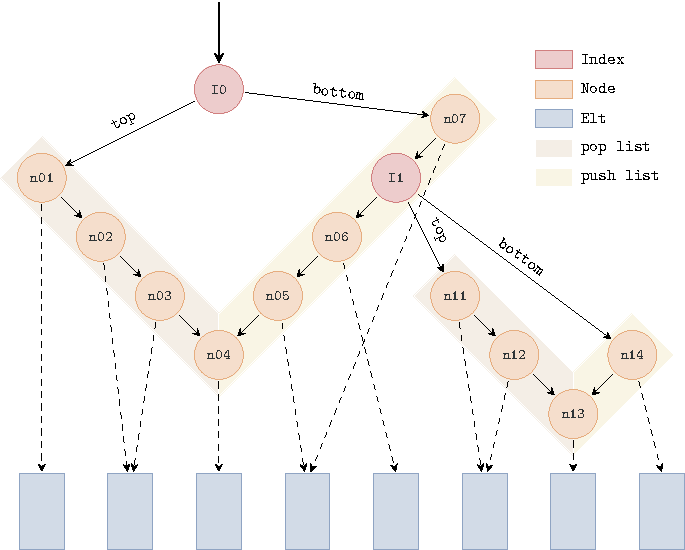
\includegraphics[scale=0.6]{queue.pdf}
\caption{Example of a possible queue internal structure. Here, the main queue is accessible through the index \code{I0}. The index \code{I1} is pointing to a queue concatenated during a previous merge operation. This queue will be unfolded during the next normalization. Because of the \irmin store behavior,  two nodes containing the same element share its physical representation.}
\label{queuegraph}
\end{figure}

\paragraph{Major operations}
The two first main operations on a queue are push and pop.
The push operation adds a new \code{Elt} containing the pushed value, and a \code{Node} pointing to this element and the previous bottom element of the queue.
It return a new \code{Index} where the bottom element is the new created \code{Node}.
The pop operation try to read the top element of the queue.
If the pop list is empty, the queue is normalized.
Then it return the value associated to the reading \code{Node} and an \code{Index} where the top element is the following element of the reading \code{Node}.
On average, there is two reads and three writes in the \irmin store for one push and one pop.

The other main operation is the merging one.
The merging operation take three arguments: two queues to be merged \code{q1} and \code{q2}, and a common ancestor to those two queue called \code{old}.
The resulting queue -- called \code{new} -- has to reflect the transformations from \code{old} to both \code{q1} and \code{q2}. First, element of a \code{old} which have been removed from \code{q2} are removed from \code{q1}. This is done without accessing these element by using the \code{push} and \code{pop} values. In the same way, all elements of \code{old} which are still in \code{q2} are removed. Then, \code{q2} is concatenate at the end of \code{q1} by adding a new node where the field \code{branch} contain the index of \code{q2}. In the worst case the merge operation uses a number of read linear in the size of \code{old}, but always only one write.



\subsection{Ropes}

\begin{figure}[hbt]
\centering
\setlength{\tabcolsep}{1cm}
\begin{tabular}{|c|c|c|}
\hline
	Operation &
	Rope &
	String \\
\hline
	Set/Get &
	\cellcolor{butter!20} $O(\log n)$ &
	\cellcolor{chameleon!20} $O(1)$ \\
\hline
	Split &
	\cellcolor{butter!20} $O(\log n)$ &
	\cellcolor{chameleon!20} $O(1)$ \\
\hline
	Concatenate &
	\cellcolor{butter!20} $O(\log n)$ &
	\cellcolor{scarletred!20} $O(n)$ \\
\hline
	Insert &
	\cellcolor{butter!20} $O(\log n)$ &
	\cellcolor{scarletred!20} $O(n)$ \\
\hline
	Delete &
	\cellcolor{butter!20} $O(\log n)$ &
	\cellcolor{scarletred!20} $O(n)$ \\
\hline
\hline
	Merge &
	\cellcolor{chameleon!20} $\log\left(f(n)\right)$ &
	\cellcolor{butter!20} $f(n)$ \\
\hline
\end{tabular}
\caption{Comparison of the complexity of several operations on ropes and strings. $n$ denotes the length of the rope/string, and $f$ is the complexity of the merge function provided by the user.}
\label{complexitytable}
\end{figure}

\paragraph{General description}
A rope is a data structure that is used for efficiently storing and manipulating a very long string.
A rope is a binary tree having leaf nodes that contain a short string.
Each node has an index equal to the sum of the length of each strings in its left subtree.
Thus a node with two children divides the whole string into two parts: the left subtree stores the first part of the string and the right subtree stores the second part.
The binary tree can be seen as several levels of nodes.
The bottom level contains all the nodes that contain a string when higher levels have fewer and fewer nodes.
The top level consists of a single \emph{root} node.

The main operations on a rope are \emph{set}, \emph{get}, \emph{split}, \emph{concatenate}, \emph{insert} and \emph{delete}. Set and get respectively set or get the character at a given position. Split$(t, i)$ split at the position $i$ the rope $t$ into two new rope. Concatenate$(t_1, t_2)$ return a new rope which is the concatenation of $t_1$ and $t_2$. Insert$(t, i, s)$ insert the character chain $s$ in the rope $t$ at the position $i$. Finally, Delete$(t, i, j)$ delete in the rope $t$ the characters between $i$ and $j$. The figure~\ref{complexitytable} compares the complexity of these operations for a rope and a string.

If ropes are mainly used to manipulate strings, they can also be used to manipulate any other types of container, as long as they support the above six operations.
In fact, I design the ropes with the following idea:
"give me a container with a set of operations, and I will return you a rope on this container, supporting the same operations but achieving a better complexity, with the exception of set and get".
That is why I request a merge operation on the container in order to implement the merge operation of the mergeable rope.
Indeed, because such a rope can be built on any type of container, it is impossible to have a general way to merge it.

\begin{figure}[hbt]
\centering
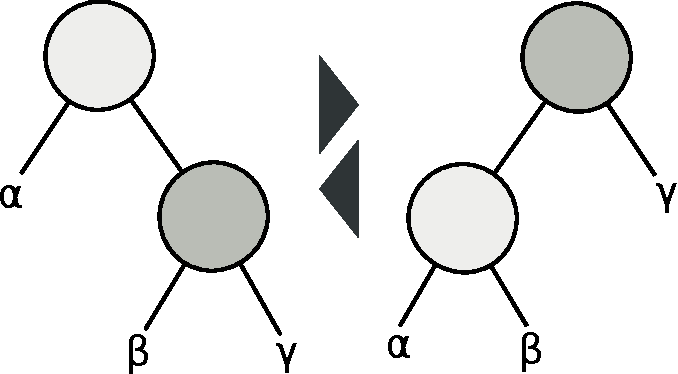
\includegraphics[scale=0.6]{rotations.pdf}
\caption{Generic tree rotation. A tree rotation moves one node up in the tree and one node down.}
\label{rotationgraph}
\end{figure}

\paragraph{Implementation overview}
The implementation of mergeable ropes is quite straightforward, in the sense that it follows the previous description.
The tree containing the rope is a self-balancing binary search tree which keep a factor two between its minimal and maximal depth.
To implement such tree, the \irmin store is specialized in order to contain three types of elements.
As in mergeable queue, \code{Index} are accessors to the data structure.
\code{Node} are intermediate element of the tree which contain informations to improve the binary search.
Finally, \code{Leaf} are the user-defined container on which the rope is built.

The implementations of the six main operations follow more or less the same pattern.
A binary search is made on the tree in order to determine the leaves concerned by the operation.
Then the operation is applied on the containers found in the leaves.
In order to achieve the $\log n$ complexity, the size of these containers has to be in the same order as the depth of the tree.
Finally, the tree is recursively rebuilt, using the rotation transformation described in the figure~\ref{rotationgraph} in order to maintain the balancing propriety.

The merge operation is a bit different.
Given two tree to be merged and their common ancestor, their keys in the \irmin store are used to determine the smallest subtrees where modifications occurred.
Then these subtrees are linearised in containers on which the user-defined merge operation is applied.
On simple trees, this approach is very efficient because the merge operation is applied on the smallest possible container.
However, the balancing propriety reduces this effectiveness.
Indeed, the internal structure of a tree can be deeply modified during a rebalancing operation, making impossible to compare potentially large subtrees.
In order to minimize the scope of rebalancing operations, the rotation function is applied as less as possible, and only on the smallest unbalanced subtree.
Due to this restriction, the impact on the merge function efficiency is proportional to the volume of modifications produced by  an operation.

\subsection{Future works}

At this stage of my internship, I have already implemented mergeable queues and ropes data structures.
In the next weeks, I first plan to improve the implementation of the mergeable ropes, which is not yet optimal.
Then I will work on a mergeable version of the priority heap data structure.
Finally, I plan to implement an hack of the \ocaml memory which will allow to use it as a database.
After that, if there is still remaining time, I will work on some concrete use case of my data structures.

\nocite{*}
\bibliographystyle{plain}
\bibliography{biblio.bib}
\newpage

\section*{Appendix}
\addtocounter{section}{1}
\setcounter{subsection}{0}
\addcontentsline{toc}{section}{Appendix}
\renewcommand{\thesubsection}{\Alph{subsection}}

\subsection{\irmin content signature\label{appendixcontent}}
\begin{lstlisting}
module type S = sig
(** Signature for store contents. *)

  include IrminIdent.S
  (** Base types. *)

  val merge: t IrminMerge.t
  (** Merge function. Raise [Conflict] if the values cannot be merged properly. *)

end

module type STORE = sig
(** Signature for store contents. *)

  include IrminStore.AO
  (** Contents stores are append-only. *)

  val merge: t -> key IrminMerge.t
  (** Store merge function. Lift [S.merge] to keys. *)

  module Key: IrminKey.S with type t = key
  (** Base functions for foreign keys. *)

  module Value: S with type t = value
  (** Base functions for values. *)

end

module Make
    (K: IrminKey.S)
    (C: S)
    (Contents: IrminStore.AO with type key = K.t and type value = C.t)
  : STORE with type t = Contents.t
           and type key = K.t
           and type value = C.t
(** Build a contents store. *)

module Rec (S: STORE): S with type t = S.key
(** Convert a contents store objects into storable keys, with the expected merge function (eg. read the contents, merge them and write back the result to get the final key). *)
\end{lstlisting}

\newpage

\subsection{Mergeable queue signature\label{appendixqueue}}
\begin{lstlisting}
module type S = sig

  include IrminContents.S
  (** The type of queues. *)

  type elt
  (** The elements of the queues. *)

  val create : unit -> t Lwt.t
  (** Create a new queue. *)

  val length : t -> int Lwt.t
  (** Return the length of the queue [t]. *)

  val is_empty : t -> bool Lwt.t
  (** Return true if the given queue [t] is empty, false otherwise. *)

  val push : t -> elt -> t Lwt.t
  (** Returns a queue with adds [value] to the end of [t]. Complexity: O(1). *)

  val pop : t -> (elt * t) Lwt.t
  (** Returns the top element and a version of the queue where it is removed. Raise [Empty] if the queue is empty. Complexity: amortized O(1). *)

  val peek : t -> (elt * t) Lwt.t
  (** Returns the top element and a version of the queue updated but inchanged. Raises [Empty] if no element is found. Complexity: O(1). *)

  val dump : t -> string Lwt.t
  (** Dump the contents of the queue. *)

end

module Make
    (AO: Irmin.AO_MAKER)
    (K: IrminKey.S)
    (V: IrminIdent.S)
  : S with type elt = V.t
\end{lstlisting}

\newpage
\glsaddall
\printglossaries

\end{document}